%   % !TEX root = ../../VIII,3_Rahmen-TeX_9-0.tex
%  
%   Band VIII, 3 N.~?? 	
%   Signatur/Tex-Datei:	LH_35_09_16_016
%   RK-Nr. 	41169
%   Textfolge: 				Text auf 16v, Zeichnung auf 16r										
%   Diagramme: 		1
%   edlabels:			0
%
%
\selectlanguage{ngerman}
\frenchspacing
%
\begin{ledgroupsized}[r]{120mm}
\footnotesize
\pstart
\noindent\textbf{Überlieferung:}
\pend
\end{ledgroupsized}
%
\begin{ledgroupsized}[r]{114mm}
\footnotesize
\pstart \parindent -6mm
\makebox[6mm][l]{\textit{L}}%
Aufzeichnung:
LH~XXXV~9, 16~Bl.~16.
%
Als Schreibblatt wiederverwendeter Teil eines Briefumschlags (ca.~15~x~6~cm.);
alle Ränder bis auf den oberen unregelmäßig beschnitten.
Zwei Seiten;
Bl.~16~v\textsuperscript{o} überliefert den Text, Bl.~16~r\textsuperscript{o} das Diagramm.
Rest eines Briefsiegels auf Bl.~16~v\textsuperscript{o}.
\pend
\end{ledgroupsized}
%%
%%
\selectlanguage{latin}
\frenchspacing
% \newpage%
\vspace{8mm}
%
\pstart\noindent
\normalsize
\lbrack16~v\textsuperscript{o}\rbrack\ 
%
\edtext{Videndum nihilne}{%
\lemma{Videndum}%
\Bfootnote{%
\textit{(1)}~nihilque %
\textit{(2)}~nihilne~\textit{L}}}
%
differentiae vel erroris \edtext{in Galilaeanis}{%
\lemma{in Galilaeanis}%
\Cfootnote{%
\protect\index{Namensregister}{\textso{Galilei} (Galilaeus, Galileus), Galileo 1564\textendash1642}%
\textsc{G.~Galilei}, %
\cite{00050}\title{Discorsi}, Giornata Quarta, Leiden 1638, S.~236\textendash288 % Leiden
%\cite{01084}\title{Discorsi}, Giornata Quarta, in \textit{Opere}, Bologna 1656, S.~180\textendash219 % Bologna
(\cite{00048}\textit{GO} VIII, S.~268\textendash313).%
}}
%
prodeat, supponendo \edtext{n\lbrack on\rbrack}{%
\lemma{}%
\Bfootnote{%
nam %
\textit{L ändert Hrsg.}}}
%
motus impressi\protect\index{Sachverzeichnis}{motus impressus} et  
%
ex gravitate orti\protect\index{Sachverzeichnis}{motus ex gravitate ortus} compositionem,%
\protect\index{Sachverzeichnis}{compositio motus}  
%
sed potius unum contra alterum. Nam si componas sequitur si qua ratione vis%
\protect\index{Sachverzeichnis}{vis} a gravitate%
\protect\index{Sachverzeichnis}{gravitas} impressa%
\protect\index{Sachverzeichnis}{vis a gravitate impressa} tolleretur, 
%
continuaturum adhuc (post ascensum%
\protect\index{Sachverzeichnis}{ascensus}) motum sursum. Res parallelogrammo%
\protect\index{Sachverzeichnis}{parallelogrammum} et triangulo  
%
repraesentabilis; cum tamen debeat tota vis assurgendi%
\protect\index{Sachverzeichnis}{vis assurgendi} a  
%
deprimente aethere\protect\index{Sachverzeichnis}{aether} consumi, quia ab illo etiam 
%
inter descendendum \edtext{data. Semper}{\lemma{data.}\Bfootnote{\textit{(1)}~Vis \textit{(2)}~Semper~\textit{L}}} 
%
in obliquo ictu%
\protect\index{Sachverzeichnis}{ictus obliquus} sumendae duae directiones\lbrack,\rbrack%
\protect\index{Sachverzeichnis}{directiones duae in ictu obliquo} perpendicularis%
\protect\index{Sachverzeichnis}{directio perpendicularis} et parallela,%
\protect\index{Sachverzeichnis}{directio parallela} et in sola perpendiculari\protect\index{Sachverzeichnis}{directio perpendicularis} resistentia\lbrack,\rbrack%
\protect\index{Sachverzeichnis}{resistentia}  
%
seu idem fit ac si ictu esset.
\pend
%
\pstart
Non videtur compositio Mot\textlangle us\textrangle%
\protect\index{Sachverzeichnis}{compositio motus}\ sola sufficere.  
%
Exemplo concursus duorum globorum%
\protect\index{Sachverzeichnis}{globus} obliqui,%
\protect\index{Sachverzeichnis}{concursus obliquus} concurrentium in unum%
\protect\index{Sachverzeichnis}{concursus obliquus duorum globorum in unum} 
%
\edtext{ipsi\lbrack s\rbrack}{%
\lemma{}%
\Bfootnote{%
ipsi %
\textit{L ändert Hrsg.}}}
%
 aequalem.
\pend 
%
\newpage % Für KZeitz: Nur notbehelf für Zeichnung
\pstart%
\normalsize%
\noindent%
\lbrack16~r\textsuperscript{o}\rbrack%
%
\edtext{}{%	%TRICK für Zeichnung
\lemma{\hspace*{1,6mm}%
\lbrack\textit{Fig.~1}\rbrack%
}\killnumber%
\Cfootnote{%
Leibniz hat den Buchstaben \textit{G} an zwei verschiedene Punkte vergeben; die Bezeichnung des zweiten Punktes ändert Hrsg.%
}}
\pend
%
\vspace{0.5em} %%%%%%%%% Diagramm 1
\centerline{%
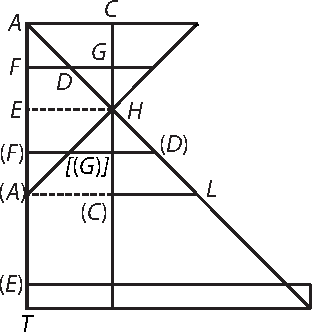
\includegraphics[width=0.36\textwidth]{%
gesamttex/edit_VIII,3/images/LH_35_09_16_016_d_016r.pdf%
}} 
\vspace{0.5em}
\centerline{%
\lbrack\textit{Fig.~1}\rbrack%
}
\count\Afootins=1200%
\count\Bfootins=1200%
\count\Cfootins=1200